\documentclass[12pt,letterpaper]{article}
\input macawlrs.tex
\newcommand{\jd}[1]{\textcolor{blue}{${\textrm{Julio: }}${#1}}}

\usepackage[scale=0.845]{geometry}


%\usepackage[urw-garamond]{mathdesign}
%\usepackage[T1]{fontenc}

%\usepackage[cmintegrals,cmbraces]{newtxmath}
%\usepackage{ebgaramond-maths}
%\usepackage[T1]{fontenc}
\usepackage{svg}

\usepackage[light,math]{iwona}

\usepackage{fancyheadings}
\usepackage{lastpage}
\lhead{\tt Deride-Ram\'irez - Working note}
\chead{\tt SNL-FRB}
\rhead{\tt \today}
\cfoot{\tt \small Page \thepage\ of \pageref{LastPage}\\ Do not circulate}

\pagestyle{fancyplain}


\usepackage{lineno}
\linenumbers

\title{A Model for Robust Regulation of Financial Networks}
\usepackage{authblk}
\author[1]{Julio Deride \thanks{julio.deride@usm.cl}}
\author[2]{Carlos Ram\'irez \thanks{carlos.ramirez@frb.gov}}
\affil[1]{Universidad T\'ecnica Federico Santa Mar\'ia, Chile}
\affil[2]{Federal Reserve Board, USA}
\renewcommand\Authands{ and }

\begin{document}
\maketitle
\baselineskip=15pt

\begin{abstract}
We develop a model to study the problem of a social planner who seeks to regulate a financial network in which shocks propagate across firms while she is unsure about the underlying network structure. We derive her optimal policy as a function of investors' attitudes towards risk and ambiguity, firms' information sets, and invariant network characteristics. Our preliminary results highlight the importance of uncertainty and firms' information sets on the optimal policy intervention.
\end{abstract}

\section{Introduction}
\section{Full information model}\label{sec:fullinfo}
Consider an economy consisting on financial institutions that hold obligations between them.  This economy is represented using a network, where each institution is represented by a node, and the corresponding obligations are represented by arcs.  Denote by $\cN=\{1,\ldots,N\}$ the set of financial institutions, and $\cA=\{e_{ij}:i,j\in\cN\}$ the set of financial obligations.  Each financial institution $i$ is concerned about their profit maximization,  by deciding an optimal level of a liquidity index \jd{A/L?, explain this}, denoted by $r_i$.

This economy faces an liquidity shock that propagates through the network, and it is modeled as a random variable $\epsilon_0\sim{\rm U}(0,b)$.  By simplicity, let's assume that this shock affects initially institution $i$ with probability $q_i$, or it affect any other institution in the network, but it propagates by a fraction $p$ of the shock to its neighbors.  Thus, the corresponding shock that institution $i$ faces, comes either from the idiosyncratic shock, or through its neighbors (or any simple-connected neighbor in the network).  Let $A$ be the adjencency matrix, i.e. $A_{i,j} = \begin{cases} 1 & (i,j)\in\cA\\ 0 &o.w.\end{cases}$, and let $\epsilon=(\epsilon_1,\ldots,\epsilon_N)$ be the vector of expected shocks.  The shock vector satisfies

\begin{equation}\label{eps}
\epsilon = S(p)\epsilon_0,\quad S(p)=\left(I +\sum_{k=1}^{N-1}p^k\tilde{A}^k\right)q,\quad \tilde{A}_1=A,\,\tilde{A}_k = A\tilde{A}_{k-1}-{\rm diag}(A\tilde{A}_{k-1})
\end{equation}

Each institution $i$ is assume to be under \emph{distress} if its liquidity index after the effect of the shock is below a given threshold $\lambda$.  Thus,
\begin{equation}\label{distress}
{\rm institution}\,i\,{\rm is\,under\,distress} \iff r_i(1-\epsilon_i) < \lambda.
\end{equation}

Additionally, we consider a benevolent financial regulator or central planner, whose goal is to maintain the stability of the financial system, while encouraging the utility maximization of each of the participants.  The only mechanism that this regulator dispose is a minimum capital requirement, that firstly, we assume that is institution-contingent.  By denoting this liquidity requirement policy by $x=(x_1,\ldots,x_N)$, and giving the propagation factor $p$, the institution $i$ solves the following optimization problem
\begin{equation}\label{imax}
r^*_i(x_i;p)\in\argmax_{r\in R_i} \lset \Ex_p\{ \pi_i(r(1-\epsilon_i))\} \mset r\geq x_i,\,\Ex_p\{\pi_i(r(1-\epsilon_i))\}\geq 0\rset,
\end{equation}
where $\epsilon_i$ comes from Equation~(\ref{eps}).  Let's consider a linear utility function, uniform for every agent, defined by
\[\pi(\tau)=\begin{cases} a_0-a_1\tau&\tau\geq \lambda\\ 0 & {\rm o.w.}\end{cases}.\]
Therefore, the expectation is given by
\begin{eqnarray*}
\Ex\{ \pi_i(r(1-\epsilon_i))\}&=&\begin{cases}
0&1-\frac{\lambda}{r}\leq 0\\
a_0-a_1r(1-\Ex\{\epsilon_i\})&\frac{1}{S_i(p)\cdot b}\left(1-\frac{\lambda}{r}\right)\geq 1\\
\frac{1}{(S_i(p)\cdot b)^2}\left(1-\frac{\lambda}{r}\right)^2\left(a_0-a_1r\left(1-\frac{1}{2}\left(1-\frac{\lambda}{r}\right)\right)\right)\,&{\rm o.w.}
\end{cases}
\end{eqnarray*}
Note that this function is continuous.  Define 
\[\lambda_i(p)=\frac{1}{1-S_i(p)\cdot b}\,\lambda, \quad \bar{\epsilon}=\Ex\{\epsilon_0\}=\frac{b}{2},\quad r^u=\frac{a^0}{a^1}\frac{1}{1-\bar{\epsilon}}.\]

The optimal value for $x_i\geq 0$ is given by
\begin{equation}\label{optri}
r_i^*(x_i)\in\argmax_{r\in R_i} \lset \Ex_p\{ \pi_i(r(1-\epsilon_i))\}\mset r\geq x_i, \Ex_p\{ \pi_i(r(1-\epsilon_i))\}\geq 0\rset = \begin{cases}
\emptyset & x_i\geq r^u\\
\lambda_i& 0\leq x_i<\lambda_i\\
x_i& \mbox{o.w}\end{cases}
\end{equation}
The function $\Ex_p\{ \pi_i(r(1-\epsilon_i))\}$ is depicted in Figure~(\ref{figExUt}).  From here it is easy to see that the optimum of the optimization problem depends on the values of $x_i$.

\begin{figure}[htbp] 
%\begin{minipage}{1.0\textwidth}
\centering
\begin{minipage}[t]{0.49\textwidth}
%\begin{figure}[htbp] 
   \centering
   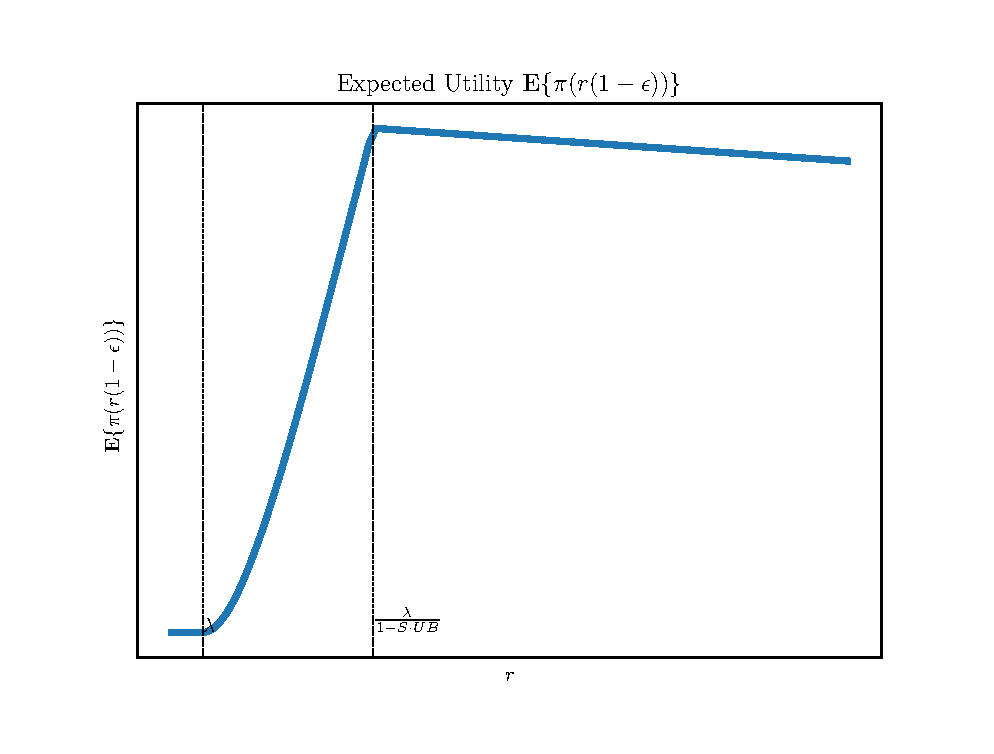
\includegraphics[width=0.95\textwidth]{Figures/ExpectedUt} 
   \caption{Expected utility}
   \label{figExUt}
%\end{figure}
\end{minipage}
\hfill
\begin{minipage}[t]{0.49\textwidth}
%\begin{figure}[htbp] %  figure placement: here, top, bottom, or page
   \centering
   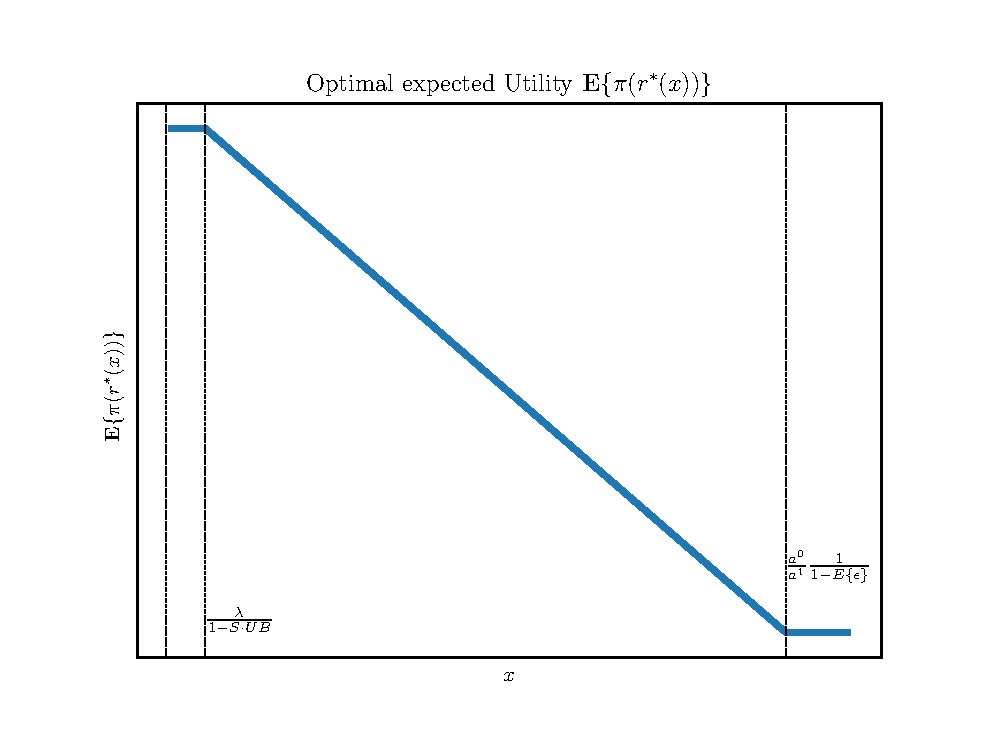
\includegraphics[width=0.95\textwidth]{Figures/OptExpUt} 
   \caption{Optimal Expected utility}
   \label{figOpExUt}
%\end{figure}
\end{minipage}
%\end{minipage}
\end{figure}

Finally, the optimal expected utility is given by
\begin{equation}\label{eqEPOpt}
\Ex_p\{\pi_i(r_i^*(x_i)(1-\epsilon_i))\}=\begin{cases}
a_0-a_1x_i(1-S_i(p)\bar\epsilon)&\lambda_i\leq x_i\leq r^u\\
a_0-a_1\lambda_i(1-S_i(p)\bar\epsilon)&0\leq x_i\leq \lambda_i\\
0&{\rm ow}
\end{cases}
\end{equation}
and it's depicted on Figure~(\ref{figOpExUt}).  It's safe to assume that the utility parameters $a_0,\,a_1$ are such that $r^u\geq 1$, and, therefore, we can dismiss the case of $r_i\geq r^u$ \jd{more on this}.  Then, the optimal policy, and optimal expected utility can be written as
\[r_i^*(x_i)=\max\{\lambda_i(p),x_i\},\quad \Ex_p\{\pi_i(r_i^*(x_i)(1-\epsilon_i))\}=a_0-a_1\max\{\lambda_i(p),x_i\}(1-S_i(p)\bar{\epsilon}).\]

\jd{comment of autoregulation on the agent's strategy.  Add the impossibility of distress. }

\subsection{Central Planner \jd{regulator?} Problem}\label{ssec:CP}
In this section we study the problem of a benevolent \jd{por supuesto!} central problem, whose main problem is to guarantee the stability of the financial network under capital shocks. The mechanism available for the Central Planner, is the minimum capital index required for each institution, i.e., this agent decides $x=(x_1,\ldots,x_N)$.  The central planner faces the problem of guaranteeing financial stability, as long as maximizing each institution's utility.  In this setting, we introduce ambiguity on the propagation parameters, i.e., the central planner has partial knowledge on the parameter $p$, that is modeled as a random variable with possible outcomes $\{p_1,\ldots,p_K\}$, with associated probabilities $\alpha_i=\Pro\{p=p_i\}$.  Denoting $\bar{p}=\Ex\{p\}$, we consider three possible objective functions, describing the goal of the central planner, based on the approach presented on \cite{Mac13alpha}
\begin{equation}\label{objcp}
f_{\theta,\gamma}(x)= \Ex_{\bar p}\Lset\sum_{i=1}^N \pi_i(r_i^*(x_i)(1-\epsilon_i))\Rset-\frac{\theta}{2}\var_{\bar p}\left(\sum_{i=1}^N\pi_i(r_i^*(x_i)(1-\epsilon_i))\right)-\frac{\gamma}{2}\var_\alpha\left(\sum_{i=1}^N\Ex_{p_i}\{\pi_i(r_i^*(x_i)(1-\epsilon_i))\}\right)
\end{equation}
This function offers a three different possibilities of analysis: first, the central planner is only concerned in maximizing the expected utility, under the expected propagation factor $\bar{p}$, secondly, the objective is to maximize the expected utility as well as minimizing the risk of the sum of utility functions, and lastly, the objective is to extend the previous case by adding a risk minimization on the ambiguity coming from the possibility of having different values of $p$.

\subsubsection{Risk-neutral Central Planner (RNCP) $(\theta=0,\gamma=0)$}
In this case, the propagation factor is fixed to $\bar p$, thus the risk-neutral central planner solves the following optimization problem
\begin{equation}\label{eq:rncp}
x^*=(x_1^*,\ldots,x_N^*)\in\argmax_{x_1,\ldots,x_N} f_{0,0}(x)=\Ex_{\bar p}\Lset\sum_{i=1}^N \pi_i(r_i^*(x_i)(1-\epsilon_i))\Rset = \sum_{i=1}^N \Ex_{\bar p} \pi_i(r_i^*(x_i)(1-\epsilon_i))
\end{equation}

The central planner can adopt two possible strategies, depending on the final goal \jd{more on this}: on one hand, impose individual capital index constraints, given by an individual policy $x_i$ for each institution. On the other hand, for information considerations, the proposed policy is a general rule, i.e., $x_i=x,\forall i$.

The solution to these two optimization problems are given by:
\begin{description}
\item[Individual policy] In this case, the problem of maximizing the function $f_{0,0}(x)$ defined in Equation~(\ref{eq:rncp}) is separable on each $x_i$, and the solution is given by
\begin{equation}\label{eq:solrncpi}
\max_{(x_1,\ldots,x_N} f_{0,0}(x)\iff x_i^*\in\argmax \Ex_{\bar{p}}\pi_i(r^*_i(x_i)(1-\epsilon_i))=[0,\lambda_i(\bar{p})],\,i=1,\ldots,N
\end{equation}

\item[Global policy] In this case, the central planner is only able to choose one value of $x$ for every institution of the financial network.  Therefore, the solution that maximizes the utility is given by
\begin{equation}\label{eq:solrncpu}
\max_{x} f_{0,0}(x)\iff x^*\in\argmax \sum_{i=1}^N \Ex_{\bar{p}}\pi_i(r^*_i(x)(1-\epsilon_i))=[0,\min_{i=1,\ldots,N}\{\lambda_i(\bar{p})\}]
\end{equation}
\end{description}
\jd{Note that this analysis always incorporates that the agents internalize the non-default condition, i.e., if the policy $x$ is too low, they natural move their optimal level to the one that avoid the default case}

\subsubsection{Risk-averse Central Planner (RACP) $(\theta>0,\gamma=0)$}
Given a parameter of risk aversion $\theta>0$, the central planner solves the following problem
\begin{equation}\label{eq:racp}
x^*\in\argmax_{x}  f_{\theta,0}(x)=\Ex_{\bar p}\left(\sum_{i=1}^N \pi_i(r^*_i(x_i)(1-\epsilon_i))\right) - \frac{\theta}{2}\var_{\bar p} \left(\sum_{i=1}^N \pi_i(r^*_i(x_i)(1-\epsilon_i))\right).
\end{equation}
In order to analyze this optimization problem, the risk-aversion term coming from the variance is written as 
\[\var_{\bar p}\left(\sum_{i=1}^N \pi_i(r^*_i(x_i)(1-\epsilon_i))\right)=\sum_{i=1}^N \var_{\bar p}(\pi_i(r^*_i(x_i)(1-\epsilon_i)))+2\sum_{j<i}\cov_{\bar p}(\pi_i(r^*_i(x_i)(1-\epsilon_i)),\pi_j(r^*_j(x_j)(1-\epsilon_j))).\]
Thus, the first computations needed are pairwise covariances.  Thus,
\begin{eqnarray*}
\cov_{\bar p}(\pi_i(r^*_i(x_i)(1-\epsilon_i)),\pi_j(r^*_j(x_j)(1-\epsilon_j)))&=&\Ex\Lset\left(a_0-a_1\max\{\lambda_i(\bar{p}),x_i\}(1-\epsilon_i)-a_0+a_1\max\{\lambda_i(\bar{p}),x_i\}(1-\bar{\epsilon_i})\right)\\
&&\quad\cdot\left(a_0-a_1\max\{\lambda_j(\bar{p}),x_j\}(1-\epsilon_j)-a_0+a_1\max\{\lambda_j(\bar{p}),x_j\}(1-\bar{\epsilon_j})\right)\Rset\\
&=&a_1^2\,S_i(\bar{p})\,S_j(\bar{p})\,\max\{\lambda_i(\bar{p}),x_i\}\,\max\{\lambda_j(\bar{p}),x_j\}\,\Ex\lset (\epsilon-\bar{\epsilon})^2\}\\
&=&a_1^2\,S_i(\bar{p})\,S_j(\bar{p})\,\max\{\lambda_i(\bar{p}),x_i\}\,\max\{\lambda_j(\bar{p}),x_j\}\,\frac{b^ 2}{12}
\end{eqnarray*}
Therefore, the objective function in Equation~(\ref{eq:racp}) is given by
\[f_{\theta,0}(x)=\sum_{i=1}^N a_0-a_1\max\{\lambda_i(\bar{p}),x_i\}(1-S_i(\bar{p})\bar{\epsilon})-\frac{\theta}{2}\frac{(a_1\,b)^2}{12}\sum_{i=1}^N\sum_{j=1}^N S_i(\bar{p})\,S_j(\bar{p})\,\max\{\lambda_i(\bar{p}),x_i\}\,\max\{\lambda_j(\bar{p}),x_j\}.\]
From this expression, it's easy to see that the the maximum of $f_{\theta,0}$ coincide with the maximum of $f_{0,0}$, as both terms are constant on the area $\{x:0\leq x_i\leq \lambda_i(\bar{p})\}$, and are decreasing outside this region.  Thus, the central planner solution for both problems, Individual and Global policy, are given by Equation~(\ref{eq:solrncpi}) and Equation~(\ref{eq:solrncpu}) respectively.


\subsubsection{Ambiguity-averse Central Planner (AACP) $(\theta=0,\gamma>0)$}
Consider the case where the Central Planner faces ambiguity with respect to the parameter $p$.  In this case, for $\theta>0$ and $\gamma>0$, the optimization problem is given by
\begin{equation}\label{eq:aacp}
x^*\in\argmax_{x}  f_{0,\gamma}(x)= f_{0,0}(x) - \frac{\gamma}{2}\var_{\alpha} \left(\sum_{i=1}^N \Ex_{\bf p}\{\pi_i(r^*_i(x_i)(1-\epsilon_i))\}\right).
\end{equation}
We follow the same strategy to compute the ambiguity term, i.e., by computing the individual covariances.  These terms are given by 
\begin{eqnarray*}
\cov_\alpha\left(\Ex_{\bf p}\pi_i(x_i),\Ex_{\bf p}\pi_j(x_j)\right)&=&a_1^2\sum_{k=1}^K \alpha_k \left(\max\{x_i,\lambda_i(p_k)\}(1-S_i(p_k)\bar{\epsilon}) - \max\{x_i,\lambda_i(\bar{p})\}(1-S_i(\bar{p})\bar{\epsilon}) \right)\\
&&\quad\quad\quad\quad\cdot\left(\max\{x_j,\lambda_j(p_k)\}(1-S_j(p_k)\bar{\epsilon}) - \max\{x_j,\lambda_j(\bar{p})\}(1-S_j(\bar{p})\bar{\epsilon}) \right)
\end{eqnarray*} 
The final form of the objective function will include a series of variance and covariance terms that decompose into piecewise linear/quadratic functions.  Thus, the central planner problem belongs to the family of nonlinear, non-concave problems, and it can be solved by using state-of-the-art global optimization solver to find the optimal value.  In the next section we explore numerical solutions to this problem for a series of financial networks.

\subsection{Examples}
\subsubsection{Toy example}
\subsubsection{\jd{Mid-size real example}}
\section{Network information asymmetries}
In this section we study the frictions induced in the regulation by information asymmetries with respect to the structure of the financial network.   In this setting, each firm only has partial information about the network.  Moreover, firm $i$ only \emph{knows} \jd{defn need a better verb} its obligations with its immediate neighbors and, therefore, the optimal capital strategy only foresees capital shocks either idiosyncratic or through one of the direct connected institution.

We extend our model from Section~(\ref{sec:fullinfo}), by replacing the adjacency matrix $A$ along with the propagation parameter $p$, with a new matrix, $E$, which represents the \emph{exposure} of each firm with respect to its neighbors, which captures adjacency and magnitude of shock propagation.  Thus, $E=(e_{ij})$, where $e_{ij}$ is the level of exposure of firm $i$ with respect to firm $j$ and, in case that firm $j$ receives a shock of $\epsilon$, then the fraction of contagion to firm $i$ is \(e_{ij}\epsilon\).  Therefore, the computation for the corresponding shock that each institution faces is given by
\begin{equation}\label{eq:epspriv}
\epsilon_i = S_i(E_{i\cdot})\epsilon_0,\quad S_i(E_{i\cdot})=(1+E')_{i\cdot}\,q=q_i+ \sum_{j\neq i} e_{ji}q_j,
\end{equation}
Note that for the computation of agent-\(i\) shock, we only require knowledge of the \(i\)-th column of the matrix $E$, i.e., only the propagation factor of the immediate neighbors of \(i\).\jd{only the incidental arrows of the directed graph}

\subsection{Individual optimal strategies}
We analyze the regulation problem following the procedure described in Section~(\ref{sec:fullinfo}).  The computations are mostly similar, but one needs to focus on the differences between the agents' problems, and the central planner problem with respect to the information available to each market participant.

For a given exposure matrix $E$, the agent profit maximization problem is given by finding an optimal capital index that maximizes the expected utility function, as given in Equation~(\ref{imax}).  Note that in this formulation, the shock that agent \(i\) faces comes from Equation~(\ref{eq:epspriv}).  The agent-\(i\) solution is given by

\begin{equation}\label{eq:privsol}
\lambda_i(E)= \frac{1}{1-S_i(E)b}\lambda,\quad r_i^*(x_i) = \max\{\lambda_i(E),x_i\},\quad \Ex_E\{\pi_i(r_i^*(x_i)(1-\epsilon_i))\}=a_0-a_1r_i^*(x_i)(1-S_i(E)\bar\epsilon)
\end{equation}

Discrepancies between the previous case only comes from the differences in the computation of the shock propagation factor \(S\), but the final form of the reaction function and the expected utility remains the same.  In the next subsection, more drastic changes are presented on the regulator problem.

\subsection{Central planner with full network information}
Following the same approach as in \S~(\ref{ssec:CP}), the central planner maximizes the sum of the expected utility of each agent, given by the function~(\ref{objcp}), by imposing a minimum capital requirement for each institution. Compared to the previously exposed approach, a fundamental difference arises: the network information available for the policy maker.  Here, for a given exposure matrix \(E\), the entire network structure enters to the shock propagation computation, that takes the following form
\begin{equation}\label{eq:cpasy}
\epsilon = S^{CP}(E)\epsilon_0,\quad S^{CP}(E)=\left(I+\sum_{k=1}^{N-1}\tilde{E}_k\right)\,q,\quad \tilde{E}_0=E',\,\tilde{E}_k=E'\tilde{E}_{k-1}-{\rm diag}(E'\tilde{E}_{k-1})
\end{equation}
This factor $S^{CP}_i$ is the updated exposure factor that incorporates network propagation of the idiosyncratic shock, and it is easy to see that $S^{CP}_i(E)\geq S_i(E)$, as the later only includes the first order term on the sum in Equation~(\ref{eq:cpasy}).  This observation leads to discrepancies in the expected critical capital requirement $\lambda_i(E)$, which will have the following form from the central planner perspective
\[\lambda_i^{CP}(E)= \frac{1}{1-S_i^{CP}(E)b}\lambda.\]
From here, it is easy to see that the critical lambda that the central planner assigns 

\subsubsection{Risk-neutral Central planner \(\theta=0,\,\gamma=0\)}
The maximization of the joint utility functions under a neutral risk attitude combined with the different information sets, is described by the following optimization 
\[x=(x_1,\ldots,x_N)\in\argmax_{x} \sum_{i=1}^N \Ex^{CP}\{\pi_i(r_i^*(x_i)(1-\epsilon_i))\},\]
where \(r_i^*(x_i)\) is the reaction function of each agent to the policy \(x_i\) (given by Eq.~(\ref{eq:privsol})), and \(\epsilon_i\) is given by Equation~(\ref{eq:cpasy}).  Especial attention is needed when computing the expectation, as the central planner forecasts an amplified shock, compare to the shocks that agents are expecting.  Therefore, the \(i\)-agent expected utility computed by the central planner is given by
\begin{eqnarray*}
\Ex^{CP}\{\pi_i(r_i^*(x_i)(1-\epsilon_i))\}&=&\Ex\{\pi_i(\max\{\lambda_i,x_i\}(1-S_i^{CP}\epsilon_0))\}\\
&=&\Ex\{\Ex\{\pi_i(\max\{\lambda_i,x_i\}(1-S_i^{CP}\epsilon_0))|\max\{\lambda_i,x_i\}(1-S_i^{CP}\epsilon_0)>\lambda\}\}\\
&=&\left(\frac{1}{bS_i^{CP}(E)}\left(1-\frac{\lambda}{r^*_i(x_i)}\right)\right)^2 \left(a_0-a_1\left(\frac{r_i^*(x_i)+\lambda}{2}\right)\right)
\end{eqnarray*}

  
\subsubsection{Risk-averse Central planner \(\theta>0,\,\gamma=0\)}

\subsubsection{Ambiguity-averse Central Planner \(\theta=0,\,\gamma>0\)}
Consider a central planner that , that faces ambiguity with respect to the exposure matrix that describes the network structure of the market.  Thus, the matrix \(E\) becomes a random variable taking values on the set of possible outcomes \(\{E_1,\ldots,E_L\}\), and \(\{\alpha_1,\ldots,\alpha_K\}\) are the corresponding associated probabilities.



\section{Example: Large scale network}


\nocite{*}
\bibliographystyle{plain}
\bibliography{refer}


\end{document}
